%%%%%%%%%%%%%%%%%%%%%%%%%%%%%%%%%%%%%%%%%
% Jacobs Landscape Poster
% LaTeX Template
% Version 1.0 (29/03/13)
%
% Created by:
% Computational Physics and Biophysics Group, Jacobs University
% https://teamwork.jacobs-university.de:8443/confluence/display/CoPandBiG/LaTeX+Poster
% 
% Further modified by:
% Nathaniel Johnston (nathaniel@njohnston.ca)
%
% This template has been downloaded from:
% http://www.LaTeXTemplates.com
%
% License:
% CC BY-NC-SA 3.0 (http://creativecommons.org/licenses/by-nc-sa/3.0/)
%

%----------------------------------------------------------------------------------------
%   PACKAGES AND OTHER DOCUMENT CONFIGURATIONS
%----------------------------------------------------------------------------------------
\documentclass[final]{beamer}
\usepackage[scale=1.24]{beamerposter} % Use the beamerposter package for laying out the poster
\usepackage[utf8]{inputenc}
\usepackage[ngerman]{babel}
\usepackage{fixltx2e}
\usepackage{caption}
\usepackage{graphicx}  % Required for including images
\usepackage{booktabs} % Top and bottom rules for tables
%-----------------------------------------------------------
\usetheme{confposter} % Use the confposter theme supplied with this template
%-----------------------------------------------------------
\setbeamercolor{block title}{fg=ngreen,bg=white} % Colors of the block titles
\setbeamercolor{block body}{fg=black,bg=white} % Colors of the body of blocks
\setbeamercolor{block alerted title}{fg=white,bg=dblue!70} % Colors of the highlighted block titles
\setbeamercolor{block alerted body}{fg=black,bg=dblue!10} % Colors of the body of highlighted blocks
%-----------------------------------------------------------
% Many more colors are available for use in beamerthemeconfposter.sty
%-----------------------------------------------------------
% Define the column widths and overall poster size
% To set effective sepwid, onecolwid and twocolwid values, first choose how many columns you want and how much separation you want between columns
% In this template, the separation width chosen is 0.024 of the paper width and a 4-column layout
% onecolwid should therefore be (1-(# of columns+1)*sepwid)/# of columns e.g. (1-(4+1)*0.024)/4 = 0.22
% Set twocolwid to be (2*onecolwid)+sepwid = 0.464
% Set threecolwid to be (3*onecolwid)+2*sepwid = 0.708
\newlength{\sepwid}
\newlength{\onecolwid}
\newlength{\twocolwid}
%\newlength{\threecolwid}
\setlength{\paperwidth}{48in} % A0 width: 46.8in
\setlength{\paperheight}{36in} % A0 height: 33.1in
\setlength{\sepwid}{0.024\paperwidth} % Separation width (white space) between columns
\setlength{\onecolwid}{0.300\paperwidth} % Width of one column
\setlength{\twocolwid}{0.608\paperwidth} % Width of two columns
%\setlength{\threecolwid}{0.708\paperwidth} % Width of three columns
\setlength{\topmargin}{-0.5in} % Reduce the top margin size
%-----------------------------------------------------------


\title{Der Experteneffekt: Grenzen kooperativen Lernens in der Primarstufe?} % Poster title
\author{Olga Urbaniak} % Author(s)
\institute{FU Berlin} % Institution(s)


\begin{document}
\addtobeamertemplate{block end}{}{\vspace*{2ex}} % White space under blocks
\addtobeamertemplate{block alerted end}{}{\vspace*{2ex}} % White space under highlighted (alert) blocks
\setlength{\belowcaptionskip}{2ex} % White space under figures
\setlength\belowdisplayshortskip{2ex} % White space under equations
\begin{frame}[t] % The whole poster is enclosed in one beamer frame
\begin{columns}[t] % The whole poster consists of three major columns, the second of which is split into two columns twice - the [t] option aligns each column's content to the top


\begin{column}{\sepwid}\end{column} % Empty spacer column
\begin{column}{\onecolwid} % The first column

\begin{block}{Ausgangspunkt}
Hinsichtlich der Lernleistungen  belegen Metaanalysen die positiven Effekte kooperativer Lehr- und Lernmethoden (Johnson, Johnson \& Stanne, 2000; Rohrbeck, Ginsburg-Block, Fantuzzo \& Miller, 2003; Slavin 1995). Die berichteten Effekte variieren allerdings stark, und über Wirkmechanismen des Wissenserwerbsprozesses beim kooperativen Lernen ist nur wenig bekannt. Untersuchungen mit jüngeren Schülerinnen und Schülern werden relativ selten durchgeführt. 

Ziel der Studie ist den Prozess des Wissenserwerbs beim kooperativen Lernen bei jüngeren Schülerinnen und Schülern näher zu untersuchen. Dazu wird die kooperative Methode des Gruppenpuzzles (Aronson, Blaney, Stephan, Sikes, \& Snapp, 1978) in der dritten Klassenstufe eingesetzt.
\end{block}

\begin{alertblock}{Gruppenpuzzle}
\textbf{Erarbeitunsphase} Lernstoff wird in verschiedene Teilgebiete aufgeteilt. Jede Schülerin bzw. jeder Schüler einer Klasse, die zuvor in Stammgruppen (A-D) zu vier Mitgliedern eingeteilt wurden, erarbeitet jeweils ein Teilgebiet. 

\textbf{Vermittlungsphase} die Teilgebiets-Experten wechseln in ihre jeweilige Stammgruppen zurück und geben das neu erworbene Wissen an die Nichtexperten ihrer Gruppe weiter. 

\textbf{Experteneffekt} Diskrepanz zwischen den Lernfortschritten von Experten und Nichtexperten.
\end{alertblock}


\begin{figure}
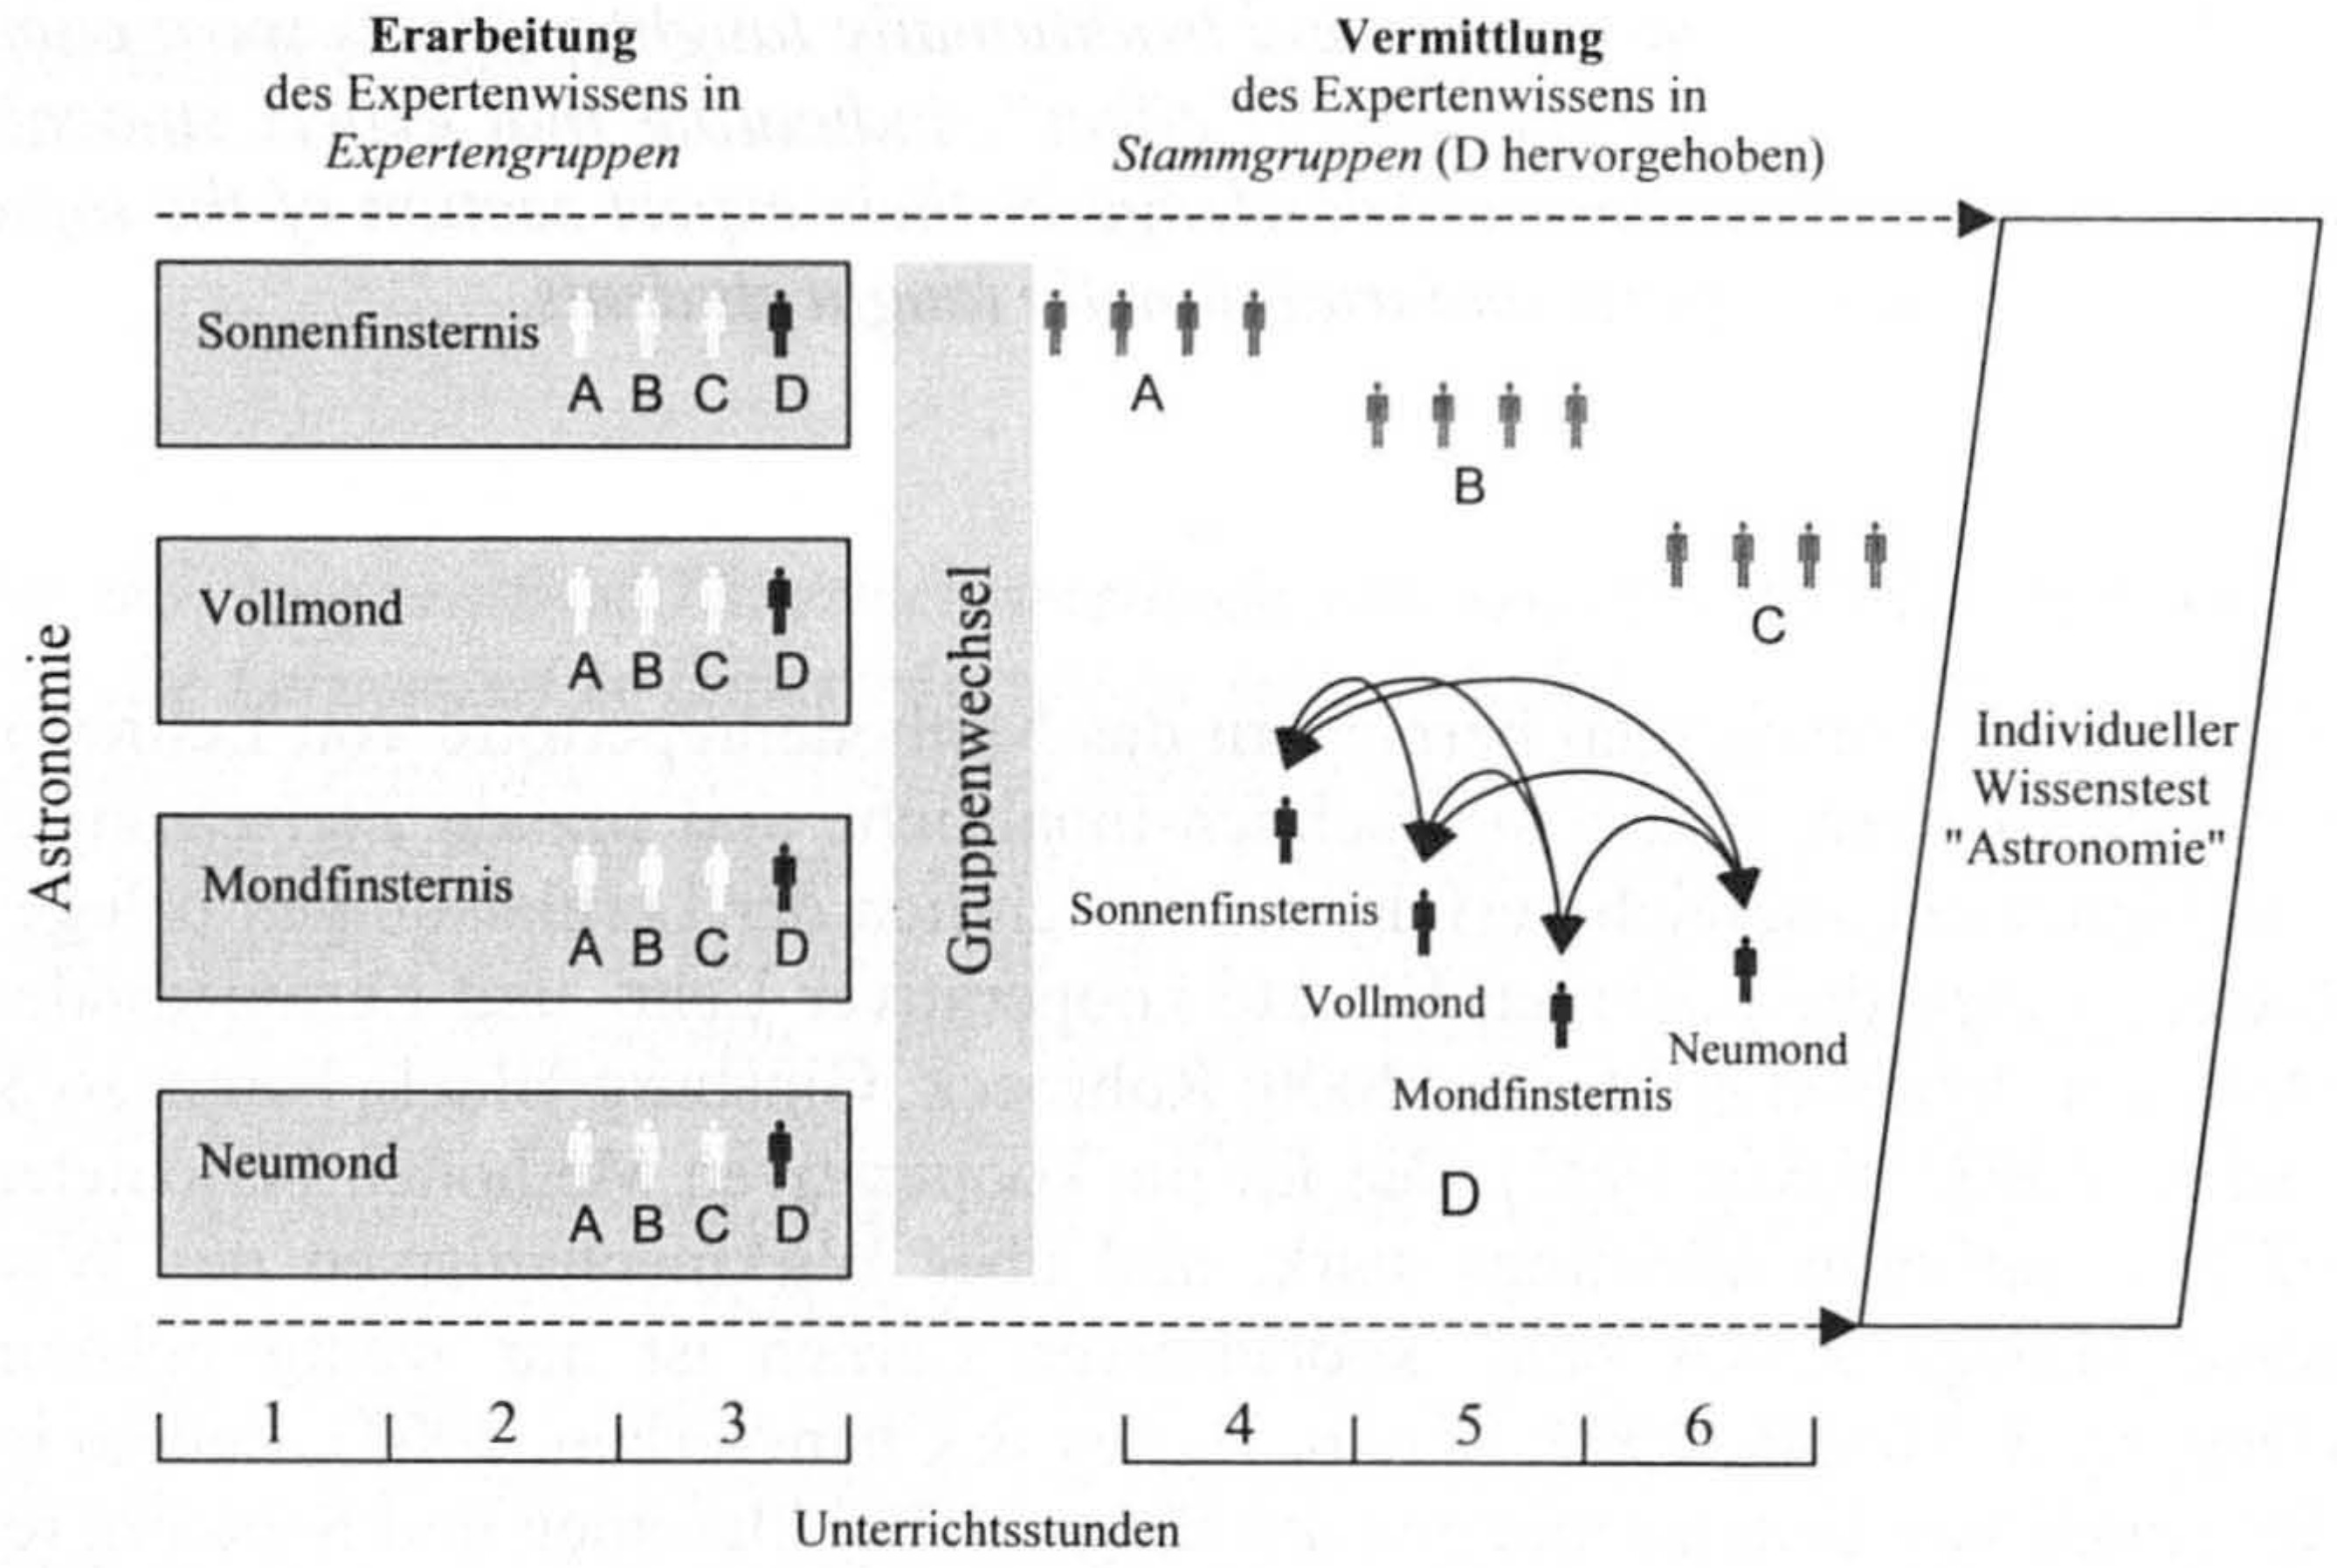
\includegraphics[width=1.0\linewidth]{experteneffekt.jpg}
\caption{Wissenserwerbsprozess im Gruppenpuzzle in einer sechsstündigen Sachunterrichtseinheit der Primarstufe}
\end{figure}


\begin{block}{Fragestellungen}
\begin{enumerate}
\item Sind die Lernleistungen der Gruppenpuzzleexperten in ihrem eigenen Expertenbereich höher als die von Nichtexperten und Kindern im herkömmlichen Unterricht in diesem Bereich?
\item Sind die Lernleistungen der Nichtexperten im Gruppenpuzzle höher als im herkömmlichen Unterricht?
\item Lässt sich das kooperative Arbeiten durch den wiederholten Einsatz der Methode verbessern?
\end{enumerate}
\end{block}


\end{column} % End of the first column
\begin{column}{\sepwid}\end{column} % Empty spacer column


\begin{column}{\twocolwid} % Begin a column which is two columns wide (column 2)
\begin{columns}[t,totalwidth=\twocolwid] % Split up the two columns wide column
\begin{column}{\onecolwid}\vspace{-.6in} % The first column within column 2 (column 2.1)


\begin{table}
\begin{tabular}{lccc}
\toprule 
 & \multicolumn{3}{c}{Studie 1} \\
\cmidrule{2-4}
 & d\textsubscript{Experten - Nichtexperten} & d\textsubscript{Experten - Kontrolle} & d\textsubscript{Nichtexperten - Kontrolle} \\
\midrule 
\textbf{Ma 1} & 0.24 & 0.37 & 0.04 \\
\textbf{Ma 2} & 0.34 & -0.02 & -0.32 \\
\textbf{Ma 3} & 0.26 & 0.41 & -0.07 \\
\midrule 
\textbf{Gesamt} & 0.28 & 0.25 & -0.12 \\
\bottomrule
\end{tabular}
{\caption*{Anm.: Positive Werte bedeuten jeweils eine Überlegenheit der vorne stehenden Gruppierung.}}
\end{table}

\end{column} % End of column 2.1


\begin{column}{\onecolwid}\vspace{-.6in} % The second column within column 2 (column 2.2)


\begin{table}
\begin{tabular}{lccc}
\toprule 
 & \multicolumn{3}{c}{Studie 2} \\
\cmidrule{2-4}
 & d\textsubscript{Experten - Nichtexperten} & d\textsubscript{Experten - Kontrolle} & d\textsubscript{Nichtexperten - Kontrolle} \\
\midrule 
\textbf{Sa l} & 0.68 & 1.21 & 0.52 \\
\textbf{Sa 2} & 0.41 & 0.23 & -0.09 \\
\textbf{Sa 3} & 0.40 & 0.79 & 0.28 \\
\textbf{Sa 4} & 1.16 & 0.29 & -0.89 \\
\textbf{Sa 5} & 0.76 & 0.35 & -0.48 \\
\textbf{Sa 6} & 0.74 & 0.72 & -0.05 \\
\midrule 
\textbf{Gesamt} & 0.69 & 0.60 & -0.12 \\
\bottomrule
\end{tabular}
{\caption*{Anm.: Positive Werte bedeuten jeweils eine Überlegenheit der vorne stehenden Gruppierung.}}
\end{table}


\end{column} % End of column 2.2
\end{columns} % End of the split of column 2 - any content after this will now take up 2 columns width


\begin{alertblock}{Auswertungsverfahren}
Als Indikatoren für den Wissenszuwachs werden die individuellen Differenzwerte zwischen Vor- und Nachkenntnisleistungen herangezogen. Um Experteneffekt überprüfen, werden für jeden Expertenbereich einer Unterrichtseinheit die mittleren Wissenszuwächse der Experten, der Nichtexperten und der lehrergeleitet Lernenden bestimmt. Da die Testwerte der Schülerinnen und Schüler in den verschiedenen Expertenbereiche nicht direkt miteinander vergleichbar sind, werden die jeweiligen Effekte über die Effektgrößen (d) bestimmt.
\end{alertblock} 


\begin{columns}[t,totalwidth=\twocolwid] % Split up the two columns wide column again
\begin{column}{\onecolwid} % The first column within column 2 (column 2.1)
%
%
%
\end{column} % End of column 2.1


\begin{column}{\onecolwid} % The second column within column 2 (column 2.2)
%
%
%
\end{column} % End of column 2.2


\end{columns} % End of the split of column 2
\end{column} % End of the second column
\end{columns} % End of all the columns in the poster
\end{frame} % End of the enclosing frame
\end{document}
